\chapter[APÊNDICE \ref{Ap:CSD}]{Cinemática dos Corpos Deformáveis}
\label{Ap:CSD}

%%==================================================================================================
%\section{Cinemática dos Corpos Deformáveis} \label{CCD}
%%==================================================================================================

Inicialmente considere um corpo deformável, idealizado como um meio contínuo que, em sua configuração inicial é denotado por $\Omega_0$ e em sua configuração atual é denotado por $\Omega$, conforme ilustrado na Figura \ref{fig:Cont}. Para se mapear os pontos que compõem o corpo em relação a uma origem preestabelecida utiliza-se $\BB{x}$ e $\BB{y}$ para denotar as coordenadas de $\Omega_0$ e $\Omega$, respectivamente. Já para se mapear $\BB{y}$ em função de $\BB{x}$ existe uma função $\BB{f}$ tal que $\BB{y}=\BB{f}(\BB{x})$, denominada como função de mudança de configuração.

\begin{figure}[h!]
    \centering
    \caption{Configurações inicial e atual de um corpo deformável.}
    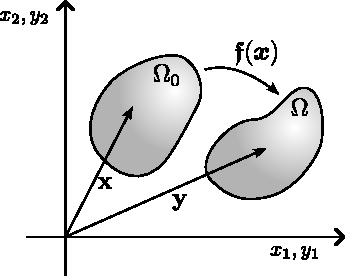
\includegraphics[width=.4\linewidth]{Figuras/Cont.pdf}
    \\Fonte: Autoria Própria (\the\year).
    \label{fig:Cont}
\end{figure}

Para um ponto $\BB{x}$ na vizinhança de $\BB{x}_0$, pode-se dizer que:

\begin{equation}
    \BB{y}(\BB{x})=\BB{f}(\BB{x}_0)+\left.\der{\BB{f}}{\BB{x}}\right|_{\BB{x}_0}\cdot d\BB{x}\text{,}
\end{equation}

\noindent em que $\BB{A}=\partial\BB{f}/\partial\BB{x}$ é o gradiente de mudança de configuração. Assim, pode-se obter uma expressão que transforme um vetor $d\BB{x}$ na configuração inicial em um vetor $d\BB{y}$ na atual:

\begin{equation}
    d\BB{y}=\BB{A}\cdot d\BB{x}\text{,}\label{eq:dyAdx}
\end{equation}

\noindent o que permite escrever o quadrado da norma de $d\BB{y}$ como:

\[
    \norm{d\BB{y}}^2=dy^2=d\BB{y}^T\cdot d\BB{y}=(\BB{A}\cdot d\BB{x})^T\cdot(\BB{A}\cdot d\BB{x})=d\BB{x}^T\cdot\BB{A}^T\cdot\BB{A}\cdot d\BB{x}
\]

Subtraindo-se $dx^2=\norm{d\BB{x}}^2$ de ambos os lados da igualdade obtém-se:

\begin{equation}
    dy^2-dx^2=d\BB{x}^T\cdot(\BB{A}^T\cdot\BB{A}-\BB{I})\cdot d\BB{x}\text{,}
    \label{eq:difdxdy}
\end{equation}

\noindent em que $\BB{I}$ é o tensor identidade de segunda ordem e $\BB{C}=\BB{A}^T\cdot\BB{A}$ é o tensor de alongamento à direita de Cauchy-Green. Dessa maneira, pode-se substituir $\BB{C}$ em \eqref{eq:difdxdy} e dividir por $2dx^2$, obtendo-se:

\[
    \frac{1}{2}\frac{dy^2-dx^2}{dx^2}=\frac{1}{2}\frac{d\BB{x}^T\cdot(\BB{C}-\BB{I})\cdot d\BB{x}}{dx^2}\text{.}
\]

\noindent Tomando um versor na direção de $d\BB{x}$ ($\BB{u}=d\BB{x}/\norm{d\BB{x}}$), tem-se que:

\begin{equation}
    \frac{1}{2}\frac{dy^2-dx^2}{dx^2}=\BB{u}^T\cdot\left(\frac{1}{2}(\BB{C}-\BB{I})\right)\cdot\BB{u}\text{.}
\end{equation}

Assim, define-se o tensor de deformações de Green-Lagrange como:

\begin{equation}
    \mathbb{E}=\frac{1}{2}(\BB{C}-\BB{I})\text{,}
    \label{eq:CSD-DefGreenLagr}
\end{equation}

\noindent que se trata de uma medida de deformação objetiva, ou seja, não registra deformações em situação de movimento de corpo rígido.

Outra medida de deformação interessante é a medida de deformação volumétrica ($\varepsilon_V$). Para isso considere o elemento infinitesimal em suas configurações inicial e atual ilustrado na Figura \ref{fig:MudVol}.

\begin{figure}[h!]
    \centering
    \caption{Mudança de volume de um elemento infinitesimal.}
    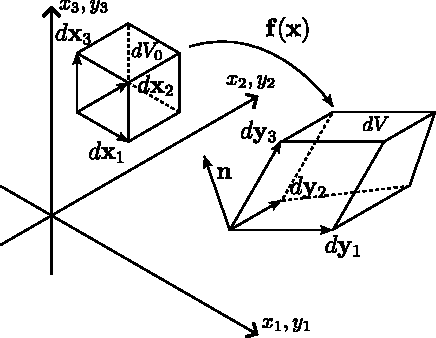
\includegraphics[width=0.5\linewidth]{Figuras/MudVol.pdf}
    \\Fonte: Autoria Própria (\the\year).
    \label{fig:MudVol}
\end{figure}

Logo o valor de $\varepsilon_V$ pode ser obtido através da relação entre o volume inicial e atual desse elemento como:

\begin{equation}
    \varepsilon_V=\frac{dV-dV_0}{dV_0}\text{.}
\end{equation}

O volume do elemento em ambas as configurações pode ser obtido por meio do produto misto dos vetores que formam o mesmo, ou seja:

\begin{subequations}
    \begin{equation}
        dV_0=d\BB{x}_1\cdot(d \BB{x}_2\times d\BB{x}_3)\text{,}
    \end{equation}
    \begin{equation}
        dV=d\BB{y}_1\cdot(d \BB{y}_2\times d\BB{y}_3)\text{,}
    \end{equation}
\end{subequations}

Conhecendo a transformação expressa em \eqref{eq:dyAdx} e fazendo as devidas simplificações pode-se obter que:

\begin{equation}
    dV=\det{(\BB{A})}dV_0=JdV_0\text{,}\label{eq:RelVol}
\end{equation}

\noindent em que $J=\det{(\BB{A})}$ é o Jacobiano da mudança de configuração.

Na sequência procura-se obter uma expressão que indique a mudança de área nas diferentes configurações. Assim, considere um cilindro infinitesimal ilustrado na figura \ref{fig:Nanson}.

\begin{figure}[h!]
    \centering
    \caption{Mudança de configuração em um cilindro infinitesimal.}
    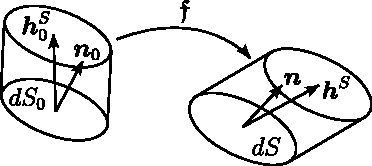
\includegraphics[width=.45\linewidth]{Figuras/Nanson.pdf}
    \\Fonte: Autoria Própria (\the\year).
    \label{fig:Nanson}
\end{figure}

Nesse contexto, a área vetorial pode ser entendida como seu valor absoluto na direção de sua normal ($d\BB{A}_0=dA_0\BB{N}$ e $d\BB{A}=dA\BB{n}$). Logo o volume do cilindro é dado pelo produto escalar da área vetorial com o vetor que define a altura do cilindro ($dV_0=d\BB{A}_0\cdot\BB{u}$ e $dV=\BB{A}\cdot\BB{v}$). Conhecendo as relações \eqref{eq:dyAdx} e \eqref{eq:RelVol}, pode-se obter que:

\begin{equation}
    \BB{n}dA=J\BB{A}^{-T}\cdot\BB{N}dA_0\text{,}\label{eq:Nanson}
\end{equation}

\noindent que é conhecida como a Equação de Nanson.

Com esse embasamento é possível apresentar os conceitos de energia nas descrições Euleriana e Lagrangiana Total. Assim, para se obter a equação do equilíbrio local de um elemento na descrição Euleriana, considere um elemento infinitesimal sujeito à ação de uma força de corpo (ou de volume) $\BB{c}$, conforme ilustrado no diagrama de corpo livre da Figura \ref{fig:CorpoLivreSolido}, que apresenta somente as forças atuantes na direção $y_1$.

\begin{figure}[h!]
    \centering
    \caption{Forças atuantes em um elemento infinitesimal na direção $y_1$.}
    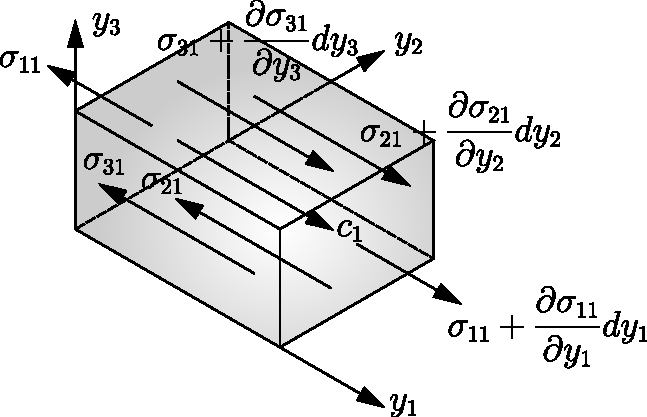
\includegraphics[width=.5\linewidth]{Figuras/CorpoLivreSolido.pdf}
    \\Fonte: Autoria Própria (\the\year).
    \label{fig:CorpoLivreSolido}
\end{figure}

Fazendo o equilíbrio das forças nessa direção e realizando as devidas simplificações tem-se:

\[\der{\sigma_{11}}{y_1}+\der{\sigma_{21}}{y_2}+\der{\sigma_{31}}{y_3}+c_1=\rho\ddot{y}_1\text{,}\]

\noindent que, expandindo analogamente para as demais direções, pode escrever nas notações simbólica (Equação \eqref{eq:EqLocEu1}) e indicial (Equação \eqref{eq:EqLocEu2}) como:

\begin{subequations}
    \begin{equation}
        \Ny\cdot\tens^T+\BB{c}=\rho\ddot{\BB{y}}\text{,}\label{eq:EqLocEu1}
    \end{equation}
    \begin{equation}
        \sigma_{ij,i}+c_j=\rho\ddot{y}_j\text{,}\label{eq:EqLocEu2}
    \end{equation}
    \label{eq:EqLocEu}
\end{subequations}

\noindent as quais representam as equações do equilíbrio local na descrição Euleriana.

Integrando a equação \eqref{eq:EqLocEu} em $\Omega$ e aplicando o teorema da divergência obtém-se:

\begin{equation}
    \int_\Gamma{\tens^T\cdot\BB{n}d\Gamma}+\int_\Omega{\BB{c}d\Omega}=\int_\Omega{\rho\ddot{\BB{y}}d\Omega}
    \text{,}
    \label{eq:EqGlobEu}
\end{equation}

\noindent onde $\Gamma=\partial\Omega$ é a fronteira do domínio de análise. Essa equação representa o equilíbrio global na descrição Euleriana.

Já em uma descrição Lagrangiana Total, será necessário transformar os termos dependentes da configuração atual para outros dependentes da configuração inicial. Assim, pode-se reescrever a Equação \eqref{eq:EqGlobEu} levando em consideração as Equações \eqref{eq:RelVol} e \eqref{eq:Nanson}:

\begin{equation}
    \int_{\Gamma_0}{J\tens^T\cdot\BB{A}^{-T}\cdot\BB{N}d\Gamma_0}+\int_{\Omega_0}{J\BB{c}d\Omega_0}=\int_{\Omega_0}{J\rho\ddot{\BB{y}}d\Omega_0}
    \text{.}
\end{equation}

\noindent Sendo $\BB{c}^0=J\BB{c}$ as forças de corpo na configuração inicial, $\rho_0=J\rho$ a densidade inicial e $\BB{P}=J\BB{A}^{-1}\cdot\tens$ o primeiro tensor de tensões de Piola-Kirchhoff, tem-se que:

\begin{equation}
    \int_{\Gamma_0}{\BB{P}^T\cdot\BB{N}d\Gamma_0}+\int_{\Omega_0}{\BB{c}^0d\Omega_0}=\int_{\Omega_0}{\rho_0\ddot{\BB{y}}d\Omega_0}\text{,}
\end{equation}

\noindent que representa a equação do equilíbrio global na descrição Lagrangiana Total.

Retornando a integral sob a fronteira $\Gamma_0$ para $\Omega_0$ por meio do Teorema da Divergência e tomando um elemento infinitesimal de volume, pode-se obter a equação do equilíbrio local na descrição Lagrangiana Total:

\begin{subequations}
    \begin{equation}
        \Nx\cdot\BB{P}^T+\BB{c}^0=\rho_0\ddot{\BB{y}}\text{, ou}
    \end{equation}
    \begin{equation}
        P_{ij,i}+c_j^0=\rho_0\ddot{y}_j\text{.}
    \end{equation}
\end{subequations}
